\setchapterpreamble[o]{%
  \dictum[Intel Corporation]{\textit{``Virtualization is a paradigm shift; it
    changes how you think about your resources.''}}}

\chapter{Introduction}
\label{cha:intro}

Virtual machine (VM) technology is a major development in computer systems
design  \cite{buzen73}.  By  providing  efficient ``copies''  of  complete
computer systems, it has  extended the multi-access, multi-programming and
multi-processing   systems  to  be   multi-environment  systems   as  well
\cite{goldberg73}.

Today's  personal   computer  systems  are  powerful   enough  to  provide
virtualization  technology which  has  long time  been  reserved for  high
performance mainframe systems only.  The paper \emph{Analysis of the Intel
  Pentium's  Ability   to  Support  a  Secure   Virtual  Machine  Monitor}
\cite{robin00analysis} discusses the problems  of how virtual machines can
be efficiently supported by the IA32 architecture.

In  the last  few years  the remote  execution of  applications  gained on
importance, because powerful server systems need not be maintained locally
anymore. They can be provided  by different organizations in a centralized
fashion.  Grid  middle\-wares  such  as Globus  \cite{globus}  or  Unicore
\cite{unicore} are examples for  execution environments in which users can
send their computation to some remote computer.

In current grid environments it is  always a problem of how an application
is referenced  by a  user.  To  actually run an  application on  a remote
resource,  the  application must  be  exactly  identified  either by  some
component of the middleware, or by the user itself.

The  problem with  that  is that  the  application could  be installed  in
different  locations on each  remote resource  --- if  it is  installed at
all. If  the user specifies the  exact location he  effectively limits the
number of resources to which he can submit the job. If, on the other hand,
the middleware  defines the exact location  and the user  only specifies a
logical identification,  a mapping between those  logical applications and
the actual executables must be provided.

Another problem  arises when a  single computing resource is  shared among
several jobs. The  middleware must make sure that  jobs which are assigned
to the same  resource do not disturb each other. To  make that clear, take
two jobs from  different users which are both scheduled  to be executed on
the same grid-resource. The least problem  that can occur is that one task
is unfair to the  other one (\ie it consumes too much  CPU time or memory)
--- this can be handled  by simply terminating the misbehaving process.  A
much worse  problem is a misbehaving job  that does so on  purpose. Such a
job could for instance attempt to steal confidential and private data from
other jobs without being noticed by the execution system.

This  work tackles  these problems  by providing  the user  with  a secure
execution environment that the user can setup himself. That means the user
knows for sure  that a particular application will  be available, that the
application is  actually working and  where it is located.   Each provided
execution domain  is running  in its own  dedicated virtual  machine. That
means,  a task  will not  be able  to access  any data  that belongs  to a
different task.

The   next  section   will  shortly   survey  the   reasons  why   to  use
virtualization.   After  that  an   excursion  to  the  past  and  current
virtualization technologies is taken. And finally this chapter ends with a
description of the goals of this work.

\section{Why use virtualization?}
\label{sec:benefits}

The  following  sections discuss  some  benefits  of using  virtualization
technologies  instead  of  the  conventional  approach  of  using  several
stand-alone  machines. The  various virtualization  technologies  that are
available       nowadays        are       discussed       in       section
\ref{sec:virtualization-techniques}.  The following  thoughts are based on
the  ideas  and information  that  can  be  found in  \cite{borden89}  and
\cite{virtualization-overview}.

\subsubsection{Application Development}

To  satisfy customer  demands,  not a  single,  general purpose  operating
system (\gls{glo:OS})  can be  used. Over the  time dozens  of specialized
systems have evolved --- for  instance on consumer desktop systems one can
find Apple's MacOS, Microsoft's  Windows or different Linux distributions,
just to  name a few.  On  cluster systems or dedicated  systems which must
provide  outstanding  security and  availability  other \gls{glo:OS}s  are
typically  used.\footnote{Linux  may  be  an  exception due  to  its  high
  adaptiveness}

Each  one of  those operating  systems has  been designed  to  address the
particular needs  of a large  segment of the  marketplace \cite{borden89},
but  it  also  imposes   inconveniences  for  application  developers  for
instance.   An application  that  should  be available  on  more than  one
\gls{glo:OS} has to  be not only \emph{adopted} to  each abstraction layer
an \gls{glo:OS} defines, but also \emph{tested} on each.

The testing of such an application requires an actual installation of each
target \gls{glo:OS}. The traditional approach to that was to simply take a
dedicated machine.  Virtualization however  makes it possible to have each
target \gls{glo:OS} installed on  the \emph{same machine} in parallel. The
developer  can  have  each  one   of  these  \gls{glo:OS}s  right  on  his
workstation.

\subsubsection{Server Consolidation}

Consider a  small company that wants to  take care of its  web or intranet
presence  on its  own.   This  requires at  least  three different  server
appliances: a  \gls{glo:DNS} server,  a web server  and a  database server
that supports the  latter. Three different solutions to  this problem come
into my mind.

\begin{itemize}
\item  The first one  is to  take a  single machine  which runs  all three
  appliances on top  of one operating system. The problem  in this case is
  that if  just one of the  appliances is compromised by  an intruder, the
  whole machine is compromised as well.
\item  The next  solution would  be to  deploy a  single machine  for each
  service,  \ie three  physical machines  in this  case.  This  closes the
  security  issues of  the previous  scenario, but  it leads  to increased
  costs for maintenance and administration.
\item  The  third  solution  secures  each  service  in  its  own  virtual
  environment but on  a single physical machine. This is  the best of both
  worlds.  It has  the maintenance  costs of  the first  solutions  with a
  little  overhead  in administration,  but  the  security  of the  second
  solution.
\end{itemize}

\subsubsection{Virtualization in Grid-like Environments}

A grid is a computing infrastructure in which many different resources are
connected to each other by some  kind of a network. The building blocks of
a  grid infrastructure  are called  ``fabrics''  \cite{book/Foster99}. The
fabrics  provide  different  kinds  of  resources to  the  user,  such  as
computation  resources, storage  devices or  instruments like  a satellite
dish.

Computational  jobs  that are  submitted  to  a  grid will  eventually  be
executed on one of the  computation resources. To maximize the utilization
of  computation resources,  the same  resource  could be  used to  execute
different jobs at the same  time. Additionally, the acquired resource must
be configured to support the application that is to be executed. To ensure
the  security   of  the   involved  computation  resource,   only  trusted
applications are allowed to be executed.

Virtualization technologies can  in this case be used  to allow the secure
sharing  of a given  computation resource,  while also  supporting unknown
applications.

The disadvantage of virtualization is that some overhead is imposed on the
involved system. Actually, additional abstraction layers always come along
with some  overhead. Modern processors  however are currently  evolving to
support virtualization techniques directly on the hardware.

The following section describes the history of virtualization technologies
and why they have been developed in the first place.

% The following list are reasons, why multiple operating systems may need to
% coexist and  even be used in the  same establishment at the  same time and
% how virtual machines fit into that \cite{borden89,virtualization-overview}:

% \begin{itemize}
% \item  \emph{Diverse Workload}  --- in  large establishments  it  is often
%   required, that  different computing  requirements must be  fulfilled. An
%   airport, for instance, requires  a highly responsive reservation system,
%   a  database system  for aircraft  maintenance  and parts  and a  general
%   purpose system for payroll and planning.
% \item  \emph{Test  and  development}   ---  many  companies  require  high
%   availability and stability of  their computing components, but they also
%   may want to test, develop  and deploy new software or software versions.
  
%   Here at  the Fraunhofer ITWM,  for instance, SuSE  Linux is used  as the
%   operating system for many desktop systems. To provide stability, updates
%   have to be tested prior deploying them everywhere.

%   The same holds for application  development --- a company will have some
%   productive system running the developed application, and this system has
%   to be available  24 hours a day. Clearly,  development cannot take place
%   on  the production  machines, since  the  probability of  a breakage  is
%   simply  too  high ---  machines  solely  dedicated  for development  are
%   required.
% \item \emph{Backup  and recovery} --- server  applications which represent
%   important  components   for  the  daily   work  (\eg database  systems,
%   web-servers etc.) must  be available all the time. A  nice thing to have
%   in such  a situation  is automatic recovery  from failure ---  to reduce
%   down-time two systems can be used: one of them is the productive system,
%   the  other one  is a  backup system  that is  an exact  ``copy''  of the
%   productive system  and just waits  for a failure  of the other.   Upon a
%   system failure  in the  productive system, the  backup system  will take
%   over.
% \item  \emph{Platform  independent development}  ---  over  the time  many
%   different  operating  systems have  evolved  ---  various Unix  flavours
%   (FreeBSD, Linux for  instance), DOS, Microsoft Windows, Mac  OS, just to
%   name some of them --- not all of them are compatible to each other.

%   Application developers who  want to develop an application  that runs on
%   several of these operating systems are required to port and verify their
%   application on each  target system and maybe on  several versions of the
%   same target system.

%   One way  is to have  an extra machine  with the target  operating system
%   installed on  it just for testing  and porting issues ---  that not only
%   imposes energy  costs but also maintenance  costs.

%   The other way is to use  virtual machines instead of actual machines ---
%   each virtual machine runs a version of a target operating system.
% \item  \emph{Server consolidation} ---  a common  approach for  many small
%   companies is to have one server on which runs for instance a web server,
%   some content management system with a database as its back-end under the
%   same  operating system.

%   That approach  may involve security problems,  since if just  one of the
%   services   contains  a   security  hole,   the  whole   system   can  be
%   compromised. Using virtual  machines for each of the  services, the only
%   system  that is  now compromised  is the  one providing  this particular
%   service.
% \end{itemize}

\section{The history of virtualization technologies}
\label{sec:virtualization-history}

The history of virtualization starts  with a paper entitled ``Time sharing
in  large,  fast  computers''  \cite{Strachey59}  written  by  Christopher
Strachey in  1959. His idea bases  on a single-CPU  system which processes
jobs one  after each  other. If  a program blocks  due to  some peripheral
access the  next program in the queue  gets started and will  be run until
the next peripheral  access occurs and so forth.   The system presents the
user with  a \emph{logical CPU} and  a scheduler assigns  this logical CPU
transparently  for   the  user  to   a  physical  CPU.   His   concept  of
``time-sharing''  is now  known  as \emph{\gls{glo:multi-programming}}  as
Christopher  Strachey states  in  a letter  to  Donald E.   Knuth in  1974
\cite{mccarthy92}.

This very simple scheduling strategy maximizes the utilization of the most
worthy resource  to that time  --- the CPU  --- and provides the  base for
current scheduling strategies such as \gls{glo:multi-tasking}.

\subsubsection{The Atlas Project}

Later on in the early 1960s, the ``Atlas project'' \cite{atlas-supervisor,
  kilburn61} --- a  joint effort between the University  of Manchester and
Ferranti~Ltd.~has  been founded.   The Atlas  computer has  been  the most
powerful  mainframe computer  in the  world  in those  days.  It  provided
spooling   mechanisms   and   pioneered   in  \emph{demand   paging}   and
\emph{supervisor  calls},  they  also invented  ``\gls{glo:virtmem}''  ---
called ``one-level store'' in the Atlas system.

The  supervisor calls  where activated  through interrupt  routines  or by
so-called   \emph{\gls{glo:extracode}}  instructions   within   an  object
program.  Atlas made use of two ``virtual machines'' --- one executing the
\gls{glo:supervisor} and the other was used to run user programs.

\subsubsection{The M44/44X Project}

The IBM Watson  Research Center has been the home  for the M44/44X Project
in the  mid 1960s. The goal of  this project was to  evaluate the upcoming
concepts of \gls{glo:time-sharing} \cite{denning81}.

The research team, led by R.~A.~Nelson, developed a way of partitioning an
IBM 7044 machine into sub-machines that  were each images of the 7044 with
less memory  --- the  main machine was  called M44, the  sub-machines 44X,
thus the project's name.

Especially David  Sayre and Belady made extensive  experimental studies to
evaluate the  performance of  \gls{glo:virtmem}, load control  and various
scheduling policies \cite{Belady66,denning81}.

\subsubsection{IBM virtual machines and the ``virtual machine monitor''}

IBM    has   perhaps   been    the   most    important   force    in   the
\gls{glo:virtualization}  area.   A number  of  IBM-based virtual  machine
systems were developed: the CP-40  (for a modified version of IBM 360/40),
the CP-67 (for  the IBM 360/67) and of course the  famous VM/370, and many
more \cite{creasy81,popek74}.

The  VM/370 is  the name  for three  operating systems,  the \emph{Control
  Program}  (CP),  \emph{Conversational  Monitor  System}  (CMS)  and  the
\emph{Remote Spooling and Communications Subsystem} (RSCS) \cite{creasy81}.
Together they provide a way to form virtual machines, which can be used by
many users. The CP therefore  simulates multiple copies of the hardware on
which it is running.  The CMS is the operating system which runs in such a
``virtual machine'' and provides access for the users.

These  virtual  machines  were   typically  identical  ``copies''  of  the
underlying  hardware  \cite{popek74}.   A  special  component  called  the
``virtual  machine  monitor'' (\gls{glo:VMM})  ran  directly  on the  real
hardware (see Figure~\ref{fig:arch-virt}).  Several virtual machines could
then be created by using the VMM to assigning parts of the hardware to the
virtual machine.

\begin{figure}[htbp]
  \centering
  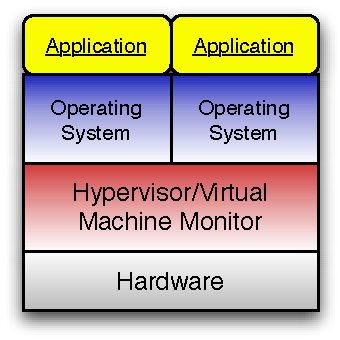
\includegraphics[scale=.75]{architecture-with-virtualization}
  \caption[Virtualization  architecture]{The bare-metal  virtualization: A
    virtual machine monitor runs as small ``operating system'' on the real
    hardware and provides access for virtual machines.}
  \label{fig:arch-virt}
\end{figure}

The virtual machine could then run  an operating system on its own and had
only access to  those parts of the hardware that  have been made available
through  the  \gls{glo:VMM}.  By  this,  new  operating  systems could  be
developed  and  tested in  a  stable  and  secure manner.   Actually,  the
\gls{glo:VMM}  itself  ran  as  a  client  to  another  \gls{glo:VMM}  for
debugging purposes.

This  kind   of  virtualization  is  called   ``full''  or  ``bare-metal''
virtualization, because an operating system that runs in a virtual machine
instance provided  by the  \gls{glo:VMM} actually thinks  it runs  on real
hardware.

\section{Virtualization Techniques}
\label{sec:virtualization-techniques}

In  contrast to  the low-level  virtualization that  was used  in  the old
mainframe   computer  systems,   today's  virtualization   approaches  are
manifold.  Virtualization is nowadays  available in all abstraction layers
that compose  a computer system, \ie  not only on the  hardware layer, but
also on the operating system and application layer.

All virtualization technologies are  backed up by the Church-Turing~Thesis
\cite{turing36,  church36}. The conclusion  of this  thesis is  that every
computer  can simulate  any other  computer.  A  nice formulation  of this
thesis has been stated by \citet{church_turing_thesis}:

\begin{quotation}
  \emph{``Any real-world computation can be translated into an equivalent
    computation involving a Turing machine.''}
\end{quotation}

% In Figure~\ref{fig:arch-novirt} is  shown, how a non-virtualized environment
% may  look like  --- it  consists of  the physical  hardware,  an operating
% system running  on that hardware and  some applications running  on top of
% the operating system.

% \begin{figure}[htbp]
%   \centering
%   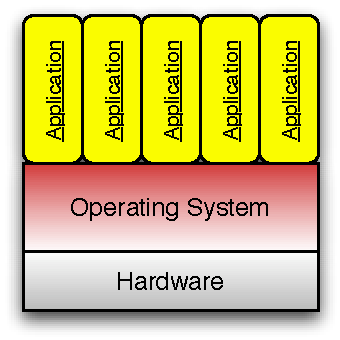
\includegraphics[scale=.75]{architecture-without-virtualization}
%   \caption[Architecture  without virtualization]{A  computer  system, that
%     does not make use of virtual machines.}
%   \label{fig:arch-novirt}
% \end{figure}

\bigskip

The  following sections  provide  a taxonomy  of  the currently  available
virtualization   technologies.   The  sections   increase  the   level  of
abstraction  step by step,  starting with  the \emph{partitioning}  of the
lowest   layer,    \ie   the    existing   hardware   and    ending   with
\emph{para-virtualization}. The latter is  based on executing machine code
partly on the physical hardware and partly by emulating the behavior.

\subsection{Partitioning}
\label{sec:vt-partitioning}

The  first  virtualization technique  bases  on  the  partitioning of  the
available physical  hardware \cite{borden89}.   It is available  since the
1960s. Two  different approaches are available, a  software based approach
and a hardware based approach.

\subsubsection{Software partitioning}
\label{sec:softw-part}

The IBM CP/67  has been the first operating  system which provided virtual
machine support, it  was running on the System/360 Model  67 and was first
available in 1967 \cite{borden89}.

As described earlier, the CP gave each user a virtual machine on which the
CMS (a  single user  operating system) was  running and provided  the user
with command processing and information management functions. Each virtual
machine was ``copy'' of the base hardware architecture, it was possible to
run OS/360 in  a virtual machine and ``in fact, even  CP/67 itself was run
"second  level" in a  virtual machine  for the  purposes of  debugging and
testing'' \cite{borden89}.

\subsubsection{Hardware partitioning}
\label{sec:hardw-part}

Hardware partitioning is an enhancement over software partitioning and was
introduced  by  the  IBM   \emph{System/370  158  MP}  and  \emph{168  MP}
systems. In 1967,  IBM introduced multiprocessor versions of  Model 65 and
67, which  provided duplexed hardware to achieve  tolerance against single
hardware failures.  By  splitting up the whole system  into two sides, two
separate systems could be created  which ran totally independent from each
other.

\subsection{Operating system-level  virtualization}
\label{sec:oper-syst-level}

This kind  of virtualization  uses the  same kernel for  the host  and all
guest systems. To  provide a guest environment with  a virtualized system,
additional support on the kernel  level is required. The guest systems run
within the  host environment  without knowing that  they do  so.  Examples
include  Solaris  Containers,  FreeBSD  and  OpenVZ.   All  three  provide
\emph{Virtual  Private  Servers} (VPSs),  \ie  completely isolated  server
environments.

FreeBSD jails are  used to shut a service or  a special server application
in its own  environment. They prohibit an application  from accessing data
that  is outside  of the  virtual environment  which an  administrator has
reserved for this jail.

\subsection{Application virtualization}
\label{sec:appl-level-virt}

The Java virtual machine \cite{java} is a well-known example for this kind
of virtualization. A program written in the Java language is compiled into
a  \emph{Java   byte  code}  and  will   be  executed  by   the  JVM  upon
execution. The virtual machine  and the operating environment together are
called the \emph{Java runtime environment}.

To  improve  execution performance,  an  additional  component called  the
\emph{Java hot-spot compiler} translates small portions of often used code
segments into  machine code (a technique  called ``dynamic translation''),
the translated code can also be cached and therefore be reused later.

\subsection{Emulation}
\label{sec:emulation}

This kind of virtualization  simulates a complete hardware architecture in
all details. By that every  operating system and therefore any application
that has been  developed for this particular architecture  can be executed
within the emulator. Some examples are:

\begin{itemize}
\item  \emph{Wine \cite{wine}}  --- Wine  is  not quite  an emulator,  but
  nonetheless I put it in this list, too. It emulates the Windows API, but
  executes many functions directly  on the underlying x86 hardware without
  emulating each instruction.
\item \emph{Bochs  \cite{bochs}} --- this  is a very portable  open source
  IA-32 PC emulator.  Each machine  instruction will be interpreted and is
  handled in software.  This emulator may for instance be  used to run x86
  code on a PowerPC platform.
\item  \emph{QEMU  \cite{qemu}} ---  this  is  both  an emulator  and  an
  virtualizer, since  it support  two modes of  operation. As  an emulator
  each instruction  gets interpreted  as it is  the case  of \emph{bochs},
  \eg it is possible  to emulate an ARM processor on  your PC. To achieve
  better  performances a  technique called  \emph{dynamic  translation} is
  used.   Running as  a virtualizer,  QEMU is  able achieve  nearly native
  performance, since most of the instructions are directly executed on the
  host CPU --- to make this possible a kernel module (QEMU accelerator) is
  required.
\end{itemize}

The disadvantage  of a  pure emulation of  a hardware architecture  is the
rather poor  execution performance.  Each  emulated instruction has  to be
translated  into at  least two  (but  probably many  more) actual  machine
instructions  of the  host  architecture\footnote{Reading the  instruction
  that is to be emulated and  interpreting it cannot be implemented with a
  single machine instruction.}.

\subsection{Para-virtualization}
\label{sec:paravirtualization}

Typically, the  instructions (or  most of them)  of a virtual  machine are
directly  executed  on  the  underlying  physical processor  to  get  best
performance  results.  Unfortunately, some  instructions are  simply ``not
designed'' to be virtualized at all (see \ref{sec:x86-problems}) --- those
instructions  perform changes  or  query the  state  of some  part of  the
physical hardware, but need not to be run in ``privileged mode''.

All instructions  that cannot be virtualized  have to be  rewritten by the
VMM before  they get executed which  means a loss  in performance.  VMWare
\cite{vmware} for instance runs as  a stand-alone application on top of an
operating system  (supported by  some extensions to  the kernel)  and uses
this kind of  binary rewriting. Figure~\ref{fig:arch-userspace-virt} shows
a schematic  overview of such  an architecture. The host  operating system
runs  directly on  the  physical hardware,  whereas  the \gls{glo:VMM}  is
executed as an application that  runs besides other applications on top of
the operating system.

\begin{figure}[htbp]
  \centering
  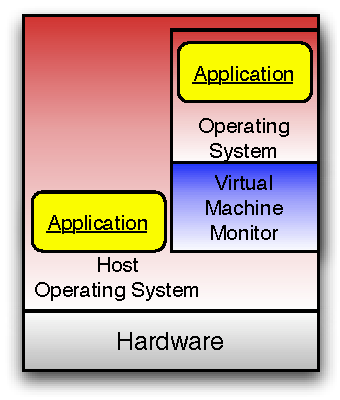
\includegraphics[scale=.75]{architecture-userspace-virtualization}
  \caption[Virtualization  in  the   user-space]{Example  for  the  VMWare
    virtualization software  which runs as  an application on top  of some
    operating system}
  \label{fig:arch-userspace-virt}
\end{figure}

The Xen hypervisor \cite{xen} however, avoids the binary rewriting problem
by providing its own ``architecture''.  A guest operating system has to be
ported       explicitly        to       this       architecture       (see
Figure~\ref{fig:arch-para-virt})  --- an operating  system which  has been
ported to  the Xen  architecture is also  called ``a Xen-aware  OS''.  The
proposed  architecture  contains  only  small modifications  to  the  real
hardware  architecture,  \ie  they  mainly modify  the  non  virtualizable
instructions.

\begin{figure}[htbp]
  \centering
  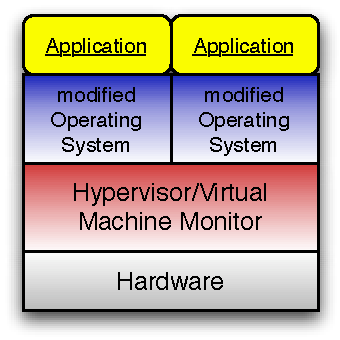
\includegraphics[scale=.75]{architecture-with-paravirtualization}
  \caption[Para-virtualization architecture]{An architecture that uses the
    para-virtualization technique}
  \label{fig:arch-para-virt}
\end{figure}

The term \emph{para-virtualization} has first been used in the description
of \emph{Denali} \cite{denali}.  In this case the VMM presents its virtual
machines with a \textbf{nearly identical} copy of the underlying hardware,
but  the virtualized  hardware  is  much less  complex  than the  physical
hardware  (no BIOS,  simpler  devices, etc.).   The  modifications to  the
virtual  hardware architecture  require  again that  the operating  system
running in a virtual machine has to be aware of those modifications.

The  disadvantage  of the  para-virtualization  technology without  binary
rewriting is  that legacy  systems cannot be  executed. These  systems are
often closed source  which means that they might not be  ported to the new
architecture at all.

The   next  section   describes  the   problems  that   arise   when  full
virtualization  (\ie   no  binary   rewriting  or  modifications   to  the
architecture) is to be used with the x86 processor architecture.

\subsection{Problems with Virtualizing the x86 Architecture}
\label{sec:x86-problems}

In \cite{schroeder72} a hardware implementation of \emph{protection rings}
is described.   These protection rings  were required for the  security of
the MULTICS  operating system. However, these  \emph{protection rings} are
still present  in today's processor  architectures, especially in  the x86
architecture.

Protection  rings are  used to  separate ``privileged''  instructions from
``unprivileged''  ones. The  x86  architecture provides  a  total of  four
rings, with ring~$0$ being the  most privileged one --- typically only two
of them  are used: ring~$0$  and ring~$3$. The  former is occupied  by the
operating  system kernel,  whereas  the  latter is  used  to execute  user
programs.  \citet{popek74} assume  a processor architecture, that provides
two modes of operation, supervisor  and user --- so the requirements which
have to be  fulfilled by an architecture to be  virtualizable apply to the
x86 architecture as  well.  They have identified three  different kinds of
instructions: privileged, sensitive and innocuous.

\begin{itemize}
\item \emph{Privileged}  instructions are those, that must  be executed in
  supervisor mode and trap if  executed in user mode. The x86 architecture
  has many  of these instructions, but  all of them  raise a \emph{general
    protection fault} if executed in user mode \cite{robin00analysis}.
  
\item \emph{Sensitive} instructions are those, that ``have a major bearing
  on     the     virtualizability     of    a     particular     machine''
  \cite{popek74}.  Generously  speaking,  they  change the  state  of  the
  hardware in some way without trapping.
  
\item \emph{Innocuous} instructions are all those which do not do any harm
  to the state of the processor from the VMM point of view.
\end{itemize}

Virtualization on the x86 architecture is typically implemented by running
the VMM in privileged mode and the virtual machines in user mode. For this
to  be successful,  all ``sensitive''  instructions \cite{popek74,popek75}
must trap into the VMM, so that they can be correctly emulated.

It  has been  analyzed that  all  privileged instructions  of the  Pentium
instruction  set correctly  trap (\ie  they raise  a  ``general protection
fault'')   and  can   be  handled   by  the   VMM  \cite{robin00analysis}.
Unfortunately    there    are    seventeen    instructions    which    are
\textbf{sensitive}  and  \textbf{unprivileged},  so  they  do  \textbf{not
  trap}.

This is the  main reason why full virtualization  has not been implemented
for  the x86  architecture for  a long  time. Intel  and AMD,  the leading
manufactures for  x86 based processors, are  currently developing hardware
support for virtualization, so that unmodified guest operating systems can
be run under a VMM.

\subsection{The Xen hypervisor}
\label{sec:xen-hypervisor}

\begin{quote}
  ``The term “hypervisor” is applied to computer systems that present a very
basic user  program interface ---  one which is  so nearly identical  to a
particular computer machine interface that an operating system intended to
support  such machines  may serve  as  a hypervisor  user program  without
software modification.'' \cite{hendricks79}
\end{quote}

\medskip

Xen \cite{xen}  is a virtualization  technology to share a  given physical
machine  using smaller  virtual machines  (\gls{glo:VM}s).  Each  of these
\gls{glo:VM}s has their own main memory, file space, access to one or more
virtual  CPUs and everything  else that  is required  to run  an operating
system (see Figure~\ref{fig:xen-architecture}).  Xen belongs to the hosted
virtualization group, which means that the \gls{glo:VMM} still requires an
operating system  to run  and does not  represent a  stand-alone operating
system itself.

\begin{figure}[ht]
  \centering
  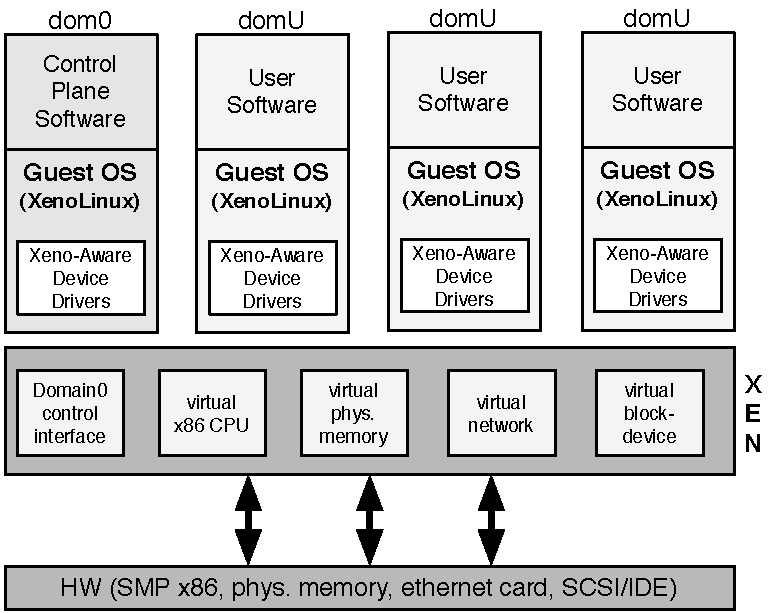
\includegraphics[scale=.75]{xen-architecture}
  \caption[Xen  architecture]{The structure  of a  system running  the Xen
    Virtual  Machine   Monitor  and  several  user   domains  (taken  from
    \cite{xen-art}).}
  \label{fig:xen-architecture}
\end{figure}

Former  versions of  the  Xen  virtual machine  monitor  did only  support
para-virtualization.   Each guest  operating system  had to  be explicitly
ported  to the  architecture  provided by  Xen.   Since version~$3.0$  Xen
supports the special hardware virtualization extensions developed by Intel
and AMD, Intel-VT and AMD-V (or Pacifica) respectively.

Xen  virtual machines  (see Figure~\ref{fig:xen-architecture})  are called
``domains''  and   the  top-level  or   most  privileged  one   is  called
\texttt{Domain-0}  --- or  \texttt{dom0} for  short ---  this is  the one,
which runs the control and management programs that are required to create
new virtual machines.  The  virtual machine instances beside \texttt{dom0}
are called ``user  domains'' --- or \texttt{domU}s for  short --- they are
less privileged and their access to the hardware is controlled and managed
by the hypervisor running in \texttt{dom0}.

The  operating system  which  is  running within  a  user domain  accesses
virtual hardware that is provided by the Xen-architecture, \eg SCSI or IDE
controllers  to  access  virtual  hard drives,  network  interface  cards,
virtual CPUs, graphic card and so on.

The following, final sections of  this chapter define the problem space of
this  work. At  first  the  problem of  executing  user-defined jobs  with
virtual machines is  illustrated by the use of  example scenarios.  I then
will  point you to  already available  products which  are similar  to the
proposed execution environment. Finally I will summarize the goals of this
work.

\section{Problem Description}
\label{sec:problem-description}

The  following two  case scenarios  are meant  to introduce  you  into the
\emph{Xen-Based  Execution Environment}. The  first scenario  represents a
typical  execution of  a  batch  job. The  second  scenario describes  the
problem of on-demand server deployment.  This is a technology that will be
provided  by grid environments  in the  future, but  is still  uncommon to
current grid environments. It describes the process of deploying a service
to key-locations within a network.

\subsection{Batch job execution}

Consider  a user  who wants  to  execute the  POV-Ray raytracing  program
\cite{POV-Ray}  on some remote  computation resource.   The input  to this
computation is  the definition of the  scene that should  be rendered. The
output of the program is a picture that shows the rendered scene.

To  submit this job  to a  grid environment,  the user  has to  define the
executable (\ie \texttt{povray}) that he  wants to use. This could be done
in a variety of ways:
\begin{itemize}
\item Each computation resource that  is connected to this particular grid
  has the application installed at the very same location.
\item The  user specifies the application  indirectly, \ie he  refers to a
  specific  application by  a logical  name. The  grid middleware  that is
  responsible  for the actual  execution (\eg  a daemon  that runs  on the
  computation  resource)  must  map  these  logical names  to  the  actual
  executables.
\item The grid provides an information service that can be queried whether
  an application is installed on a particular computation resource.
\item The user passes the executable along with her job description to the
  execution  host. This  could result  in security  problems,  because the
  application is possibly malicious. 
\item Only  platform independent applications (\eg  Java applications) are
  supported.
\end{itemize}

This list shows that many different solutions are possible just to specify
the application  that should  be executed.  The  \emph{Xen-Based Execution
  Environment} (\gls{glo:XenBEE})  approaches this problem  by putting the
application itself into an \emph{execution container}.

An  execution  container  consists  of a  stripped-down  operating  system
installation and  the application that  is to be executed.   The container
can  be made  available either  by the  user, or  by some  provider.  This
container  will then  be  used by  the  \gls{glo:XenBEE} to  create a  Xen
virtual machine instance that is  dedicated to the execution of the user's
application.   Prior  the execution  can  start  the  input data  for  the
application has to be made available. After the execution has finished the
output data has to be made available to user.


\subsection{On-demand server deployment}
\label{sec:demand-serv-depl}

Consider  for example  a group  of people  that wants  to play  an on-line
multi-player game. Such on-line games tend to require a rather low latency
network connection so that the game  can be played without having lags. If
I ran  that server on my  DSL connection with many  connected users, there
would be  large transmission delays.   This is because the  DSL connection
simply does not provide the required quality of service, \ie low latency.

The provision of  an on-demand server deployment process  could be used to
run the game server on a  well-connected remote host. The game server must
be available  within a relatively short  amount of time and  needs to stay
available for  just a couple of  hours. The hosting  environment for these
kind of servers could be provided by a rental company that has specialized
in such services.

The \gls{glo:XenBEE}  could be used to  deploy such a  server.  The server
would   be   contained    in   a   previously   prepared   \emph{execution
  container}. The game  server will then run in a  virtual machine that is
configured  with   an  appropriate   amount  of  main   memory,  computing
performance and network accessibility.

\section{Related products}
\label{ref:related-products}

The  following two  available  products provide  both  the possibility  to
deploy a virtual machine in a remote location.  To my best knowledge, they
``just'' provide the  deployment of virtual machines. They  do not provide
batch job execution semantics on their own.

\subsection{Amazon EC2}

The \emph{Amazon Elastic Computing Cloud} (EC2, \cite{amazon-ec2}) is part
of the \emph{Amazon  Web Services} project and provides  a web service for
remote execution of user provided virtual machine \gls{glo:image}s.

Amazon provides  you with  a personal storage  area where you  can deposit
arbitrary data (such as  \emph{Amazon Machine Images}). Another Amazon web
service is used  for this: the \emph{Amazon Simple  Storage Service} (S3).

With the  files that are  located in your  personal storage area,  you can
create as many virtual machines as  you like. Through web service calls or
by using one  of the various command line tools,  you can start, terminate
and monitor your deployed instances.

The  provided  environment is  very  sophisticated,  since  it provides  a
completely secure  storage area for  possibly confidential data.   It also
provides fast and on-demand deployment of the virtual machine instances.

\subsection{The XenoServer Open Platform}

The  XenoServer Open  Platform is  an implementation  of  the \emph{global
  public   computing}  paradigm   \cite{kotsovinos05}.  It   provides  the
execution of \emph{any code} from \emph{any user} \emph{anywhere}.

Servers \emph{advertise} themselves  and clients \emph{select} the servers
on which their computations or services shall be deployed. After selection
of the servers, a client send  the deployment specification to each one of
the servers. A server may then  accept or decline the request according to
local policies or resource requirements.

To integrate  this environment into  a grid, one  has to install  the grid
middleware in the deployed virtual machines.

\section{Goals of this work}
\label{sec:goals}

The previous sections have outlined the problem domain of this work. There
is  currently no  product  available which  provides  batch job  execution
semantics based on  virtual machine deployment.  One of  the goals of this
work is  to provide  such a semantic.   The following list  summarizes the
goals of the \emph{Xen-Based Execution Environment}.

\begin{itemize}
\item  \textbf{Batch job execution  semantics.} The  execution environment
  must provide support for the execution of batch jobs. That means a user
  must have  the possibility to  submit new jobs,  as well as  monitor and
  abort  his running  jobs.  The  execution  of batch  jobs requires  that
  arbitrary  input data  must be  made available  to the  job, as  well as
  generated output data must be made available to the user.

\item \textbf{On-demand server deployment.} The execution environment must
  be able to create virtual machine instances that are reachable through a
  network connection.

\item  \textbf{Integrability.}    The  execution  environment   should  be
  integrable into  existing (grid)  environments.  That means  standard or
  future  technologies  which  are  used  in  grid  environments  must  be
  supported.  This  regards the description, status  query and termination
  of jobs.

\item \textbf{Security.} Since the  execution environment could be used by
  many  different  users  at the  same  time,  it  must provide  a  secure
  execution context to user and provider.  The secure context includes the
  interaction of  a user with the  execution environment, as  well as the
  execution  of a  job. From  the provider's  point of  view  the security
  context includes authentication and  authorization of the users, as well
  as a secure communication.

\item \textbf{Efficiency.} The usage of virtual machines should not impose
  much overhead  on the total  execution time of submitted  jobs.
\end{itemize}

\subsection*{Architecture preview}

The  picture in Figure~\ref{fig:preview-architecture}  shows a  preview of
the architecture  that has been  designed and implemented in  this diploma
thesis.   In the  first  step the  user  makes his  virtual machine  image
available on some  server.  The second step depicts  the submission of the
execution  request.   Therefore a  client  and  a  server application  are
involved, \emph{xbe} and \emph{xbed} respectively.  Both are communicating
with  each other  by the  use of  a message-queue  server.   The execution
container  is retrieved  by the  \emph{xbed} in  the third  step  --- from
either a storage server, or a data  cache.  The job is executed in its own
virtual machine in the fourth step, whereas the execution is under control
of the \emph{xbeinstd} component.

\begin{figure}[ht]
  \centering
  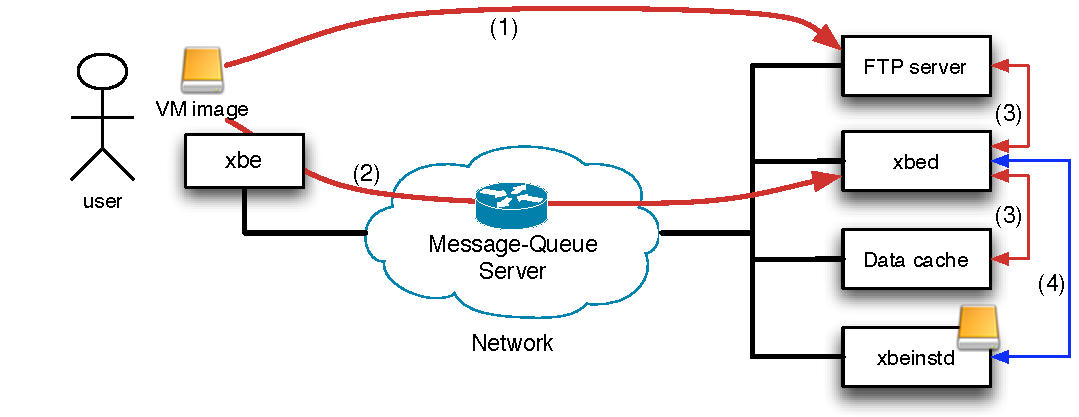
\includegraphics[scale=.75]{preview-architecture}
  \caption{Preview of the \gls{glo:XenBEE} architecture}
  \label{fig:preview-architecture}
\end{figure}

\subsection*{Structure of the following chapters}

The  remaining part  of this  work is  outlined as  follows.  In  the next
chapter, the requirements to the \gls{glo:XenBEE} are analyzed. Subsequent
to  that some basic  technologies which  have been  used to  implement the
execution  environment are  presented.  The  fourth chapter  describes the
design and implementation of the  proposed work.  The results of performed
experiments are  provided in the  fifth chapter.  The conclusions  of this
work and some directions for future  developments can be found in the very
last chapter.

%%% Local Variables: 
%%% TeX-master: "main.tex"
%%% End:
